\documentclass{article}
\usepackage{times}
\usepackage{amsmath}
\usepackage{graphicx}
\usepackage{geometry}

\begin{document}

\title{HV Pulse Capacitor Failure Analysis }
\author {Andrew D. Zonenberg, Ph.D \\ Research Scientist \\ Antikernel Labs}
\date{\today}
\maketitle

\section{Introduction}

Applied Ion Systems (AIS) requested a failure analysis of a Kemet C4540H683KGGWCT050 pulse capacitor, which had failed
catastrophically during maximum-power (2 kV) test firing of a prototype AIS-gPPT3-1C-T pulsed plasma thruster.

\begin{figure}[h]
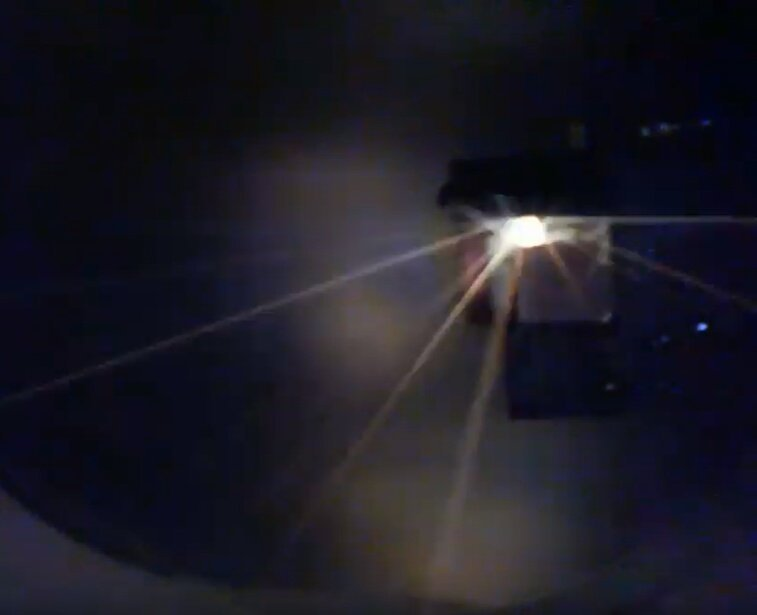
\includegraphics[scale=0.35]{cap-failure.jpg}
\caption{Video frame from test chamber at the moment of failure}
\label{failure}
\end{figure}

Antikernel Labs performed a best-effort analysis at no cost in order to support the open-hardware nature of AIS's work.

This document is licensed under Creative Commons Attribution-NonCommercial-NoDerivatives 4.0 International.

\pagebreak
\section{Specimen Overview}

Two Kemet C4540H683KGGWCT050 capacitors were provided by AIS: the failed part, as well as an identical undamaged
capacitor removed from the failed board to be used for process development and testing.

The capacitor is a 11.4 x 10.2 x 2.7 mm multi-layer ceramic capacitor (MLCC) using C0G-type dielectric, with a nominal
capacitance of 68 nF and a 2 kV voltage rating.

\begin{figure}[h]
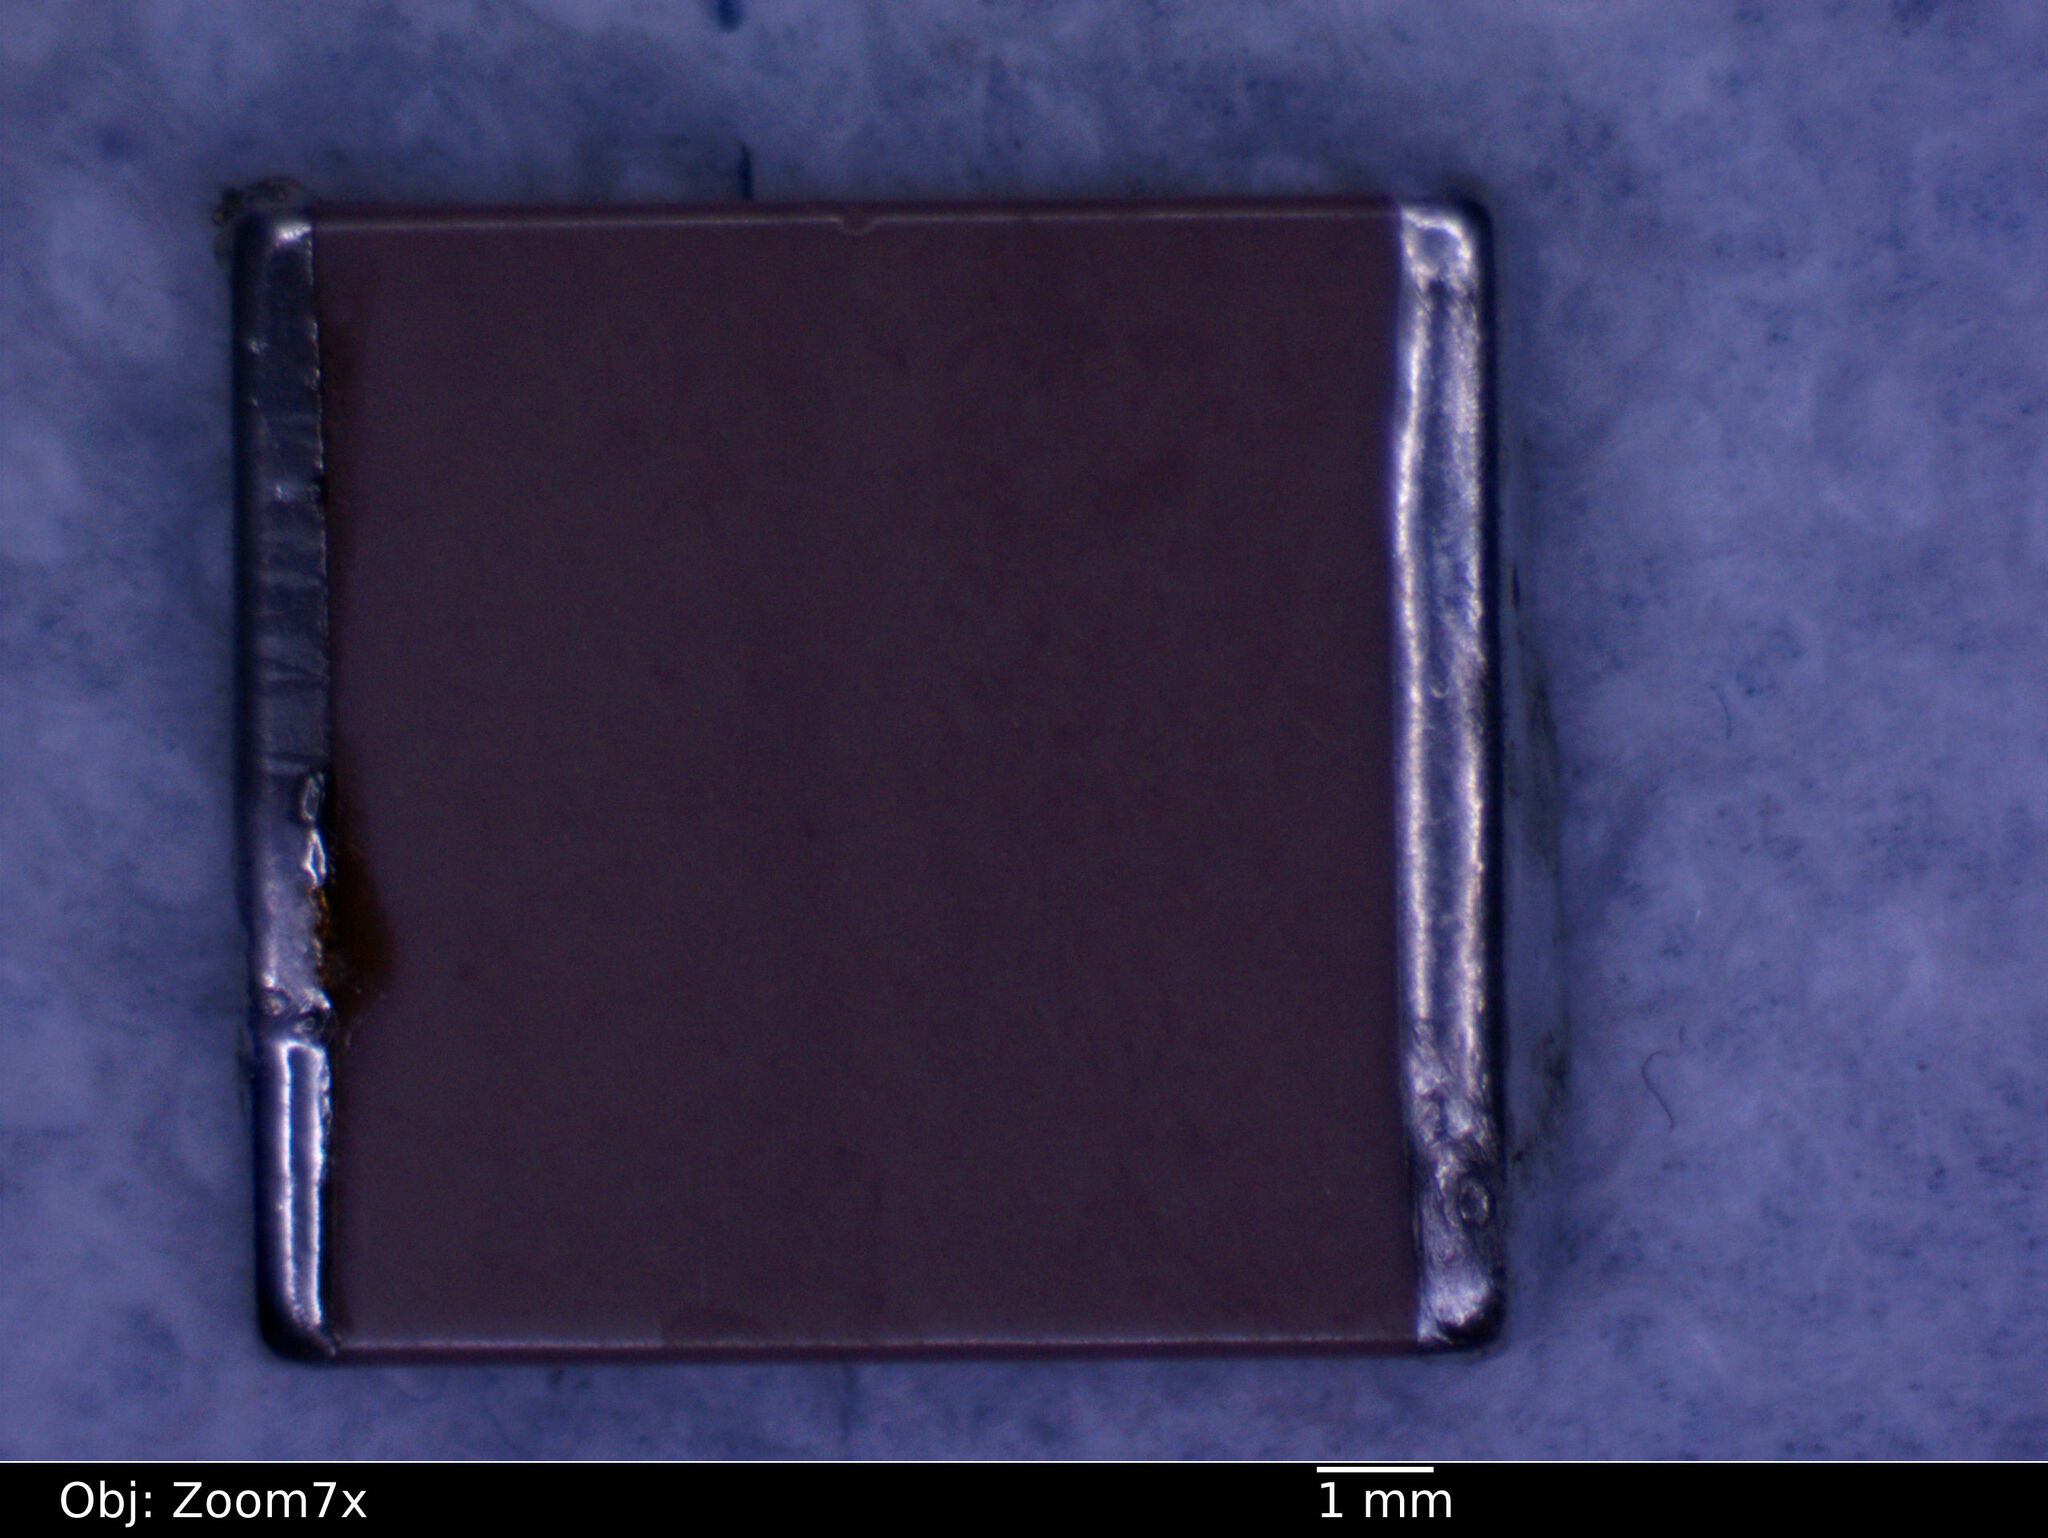
\includegraphics[scale=0.25]{01-goodcap-top_annotated.jpg}
\caption{Top view of undamaged capacitor}
\label{overview}
\end{figure}

\pagebreak
\section{Analysis}

Preliminary optical imaging of the failed side of the capacitor showed a cratered region with long cracks radiating
lengthwise down the capacitor body.

\begin{figure}[h]
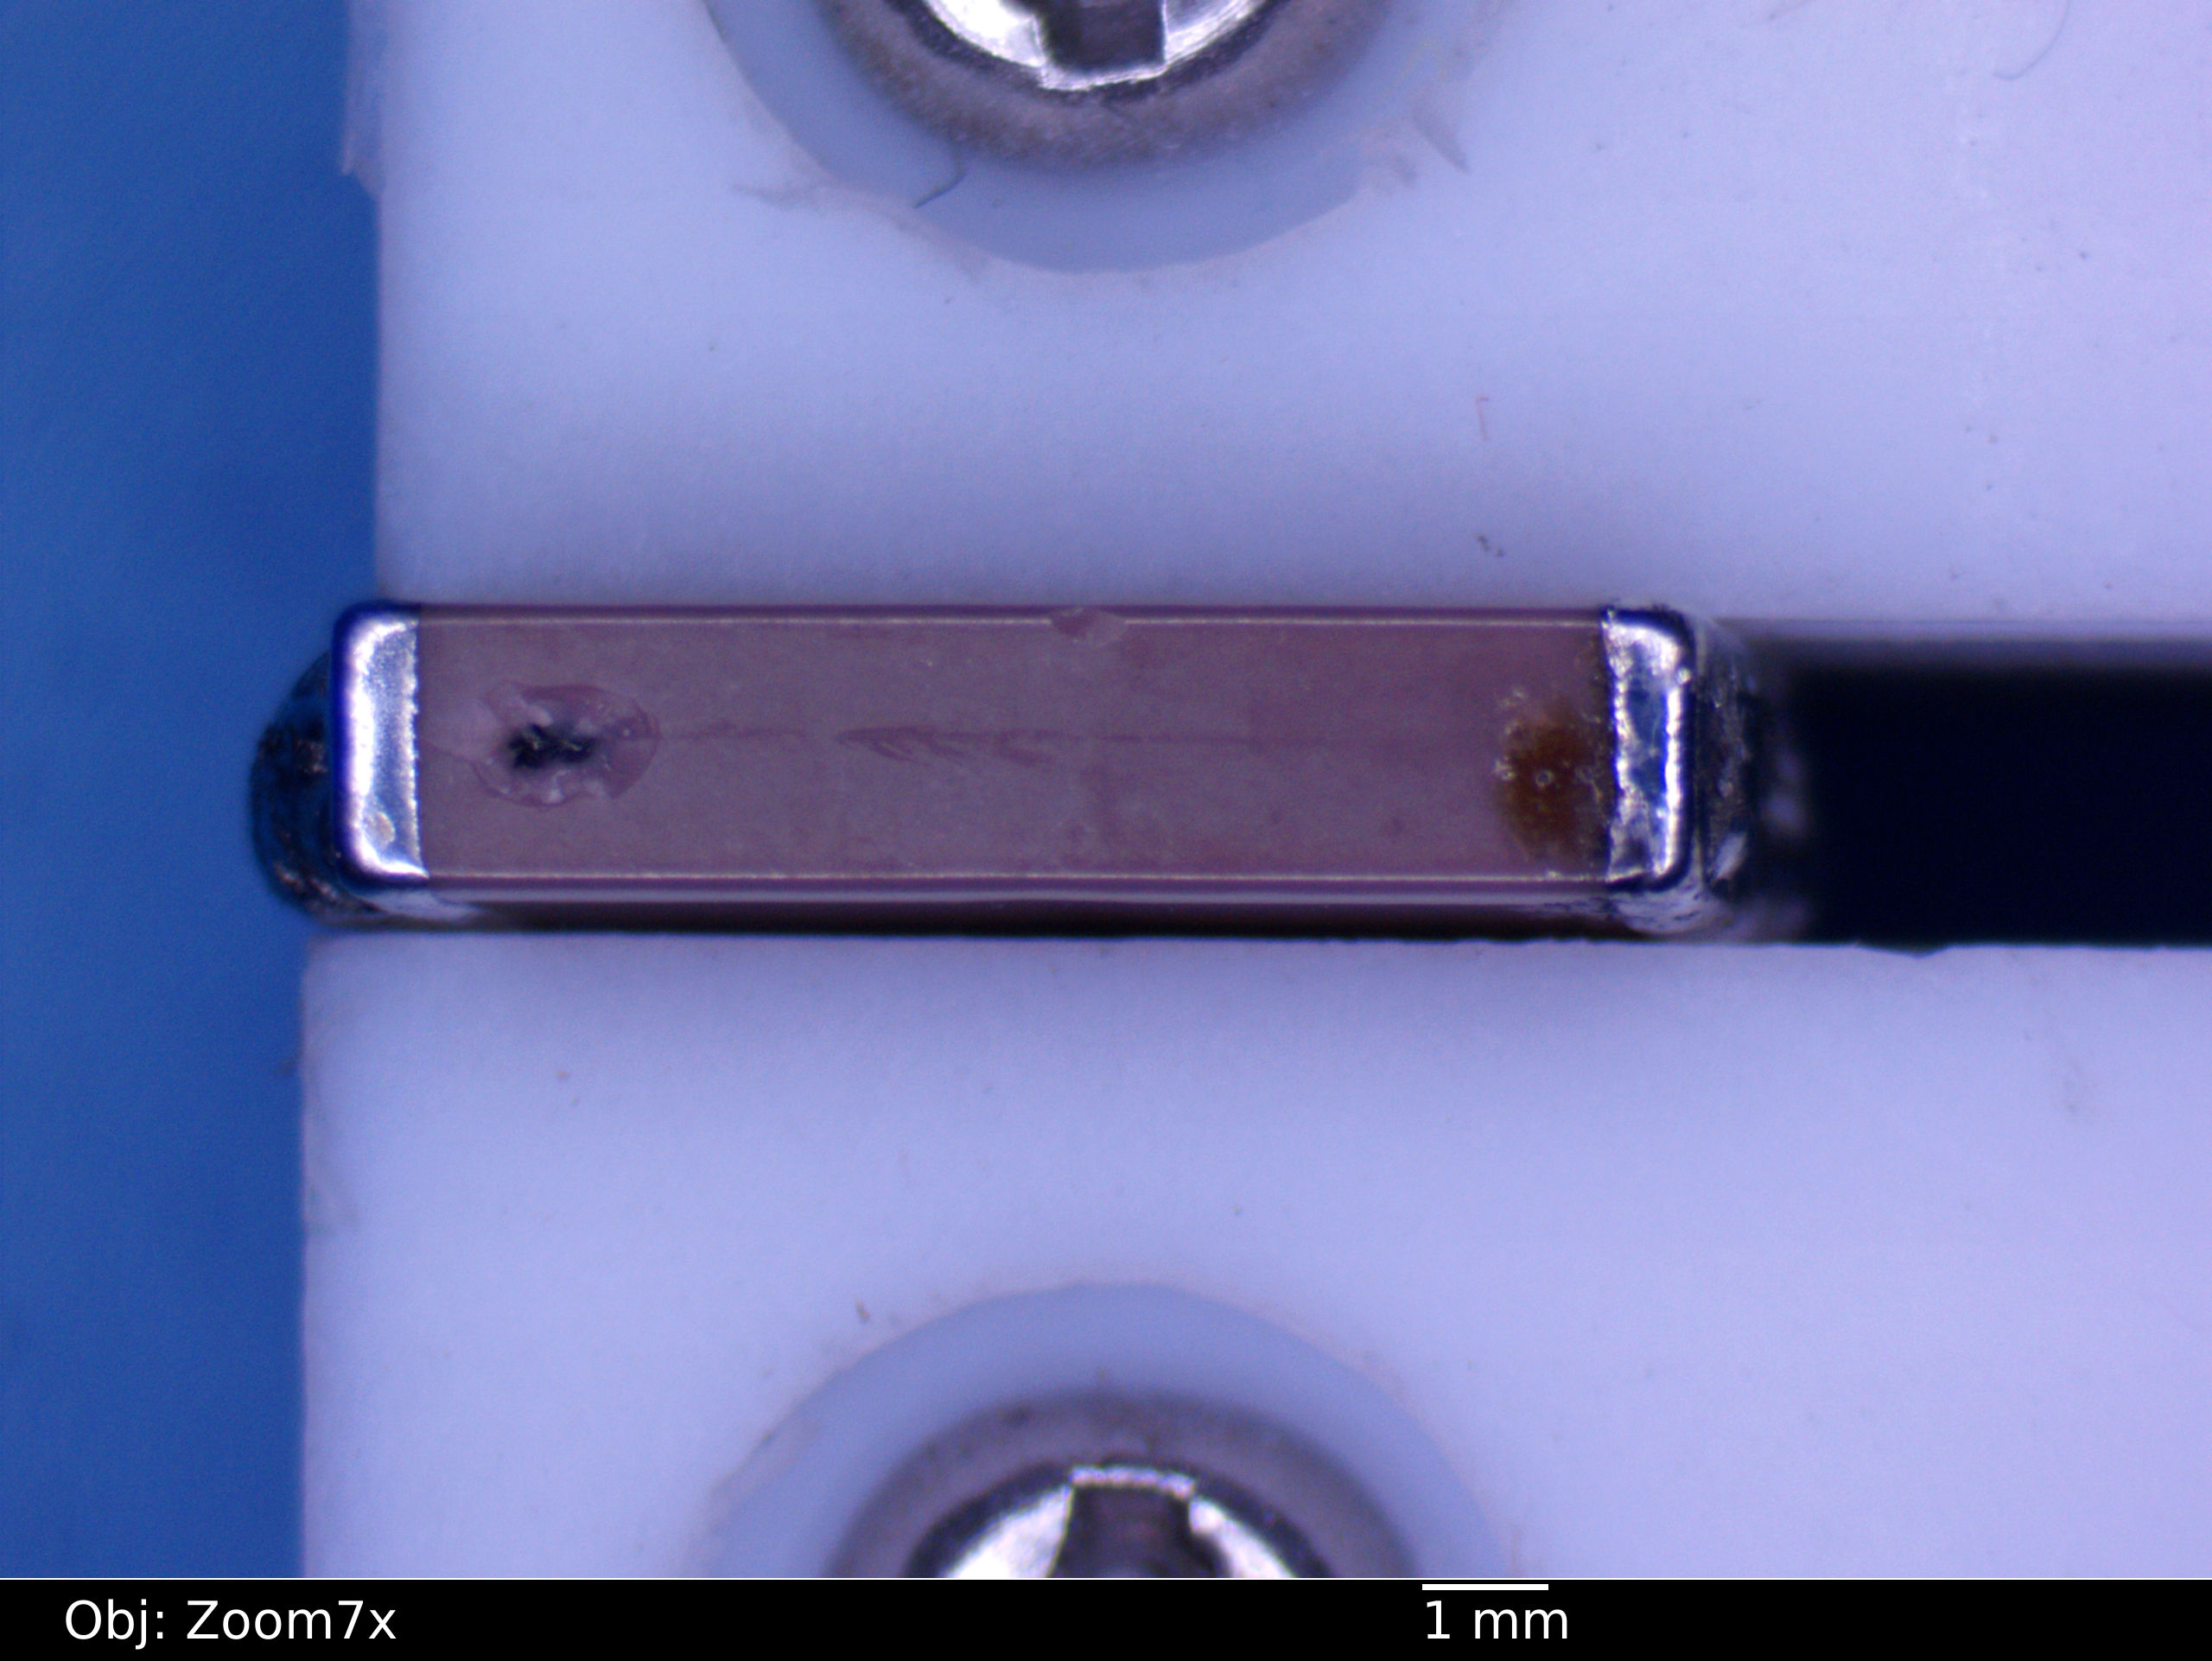
\includegraphics[scale=0.25]{02-badcap-side_annotated.jpg}
\caption{Overview of failure site}
\label{fail-overview}
\end{figure}

\begin{figure}[h]
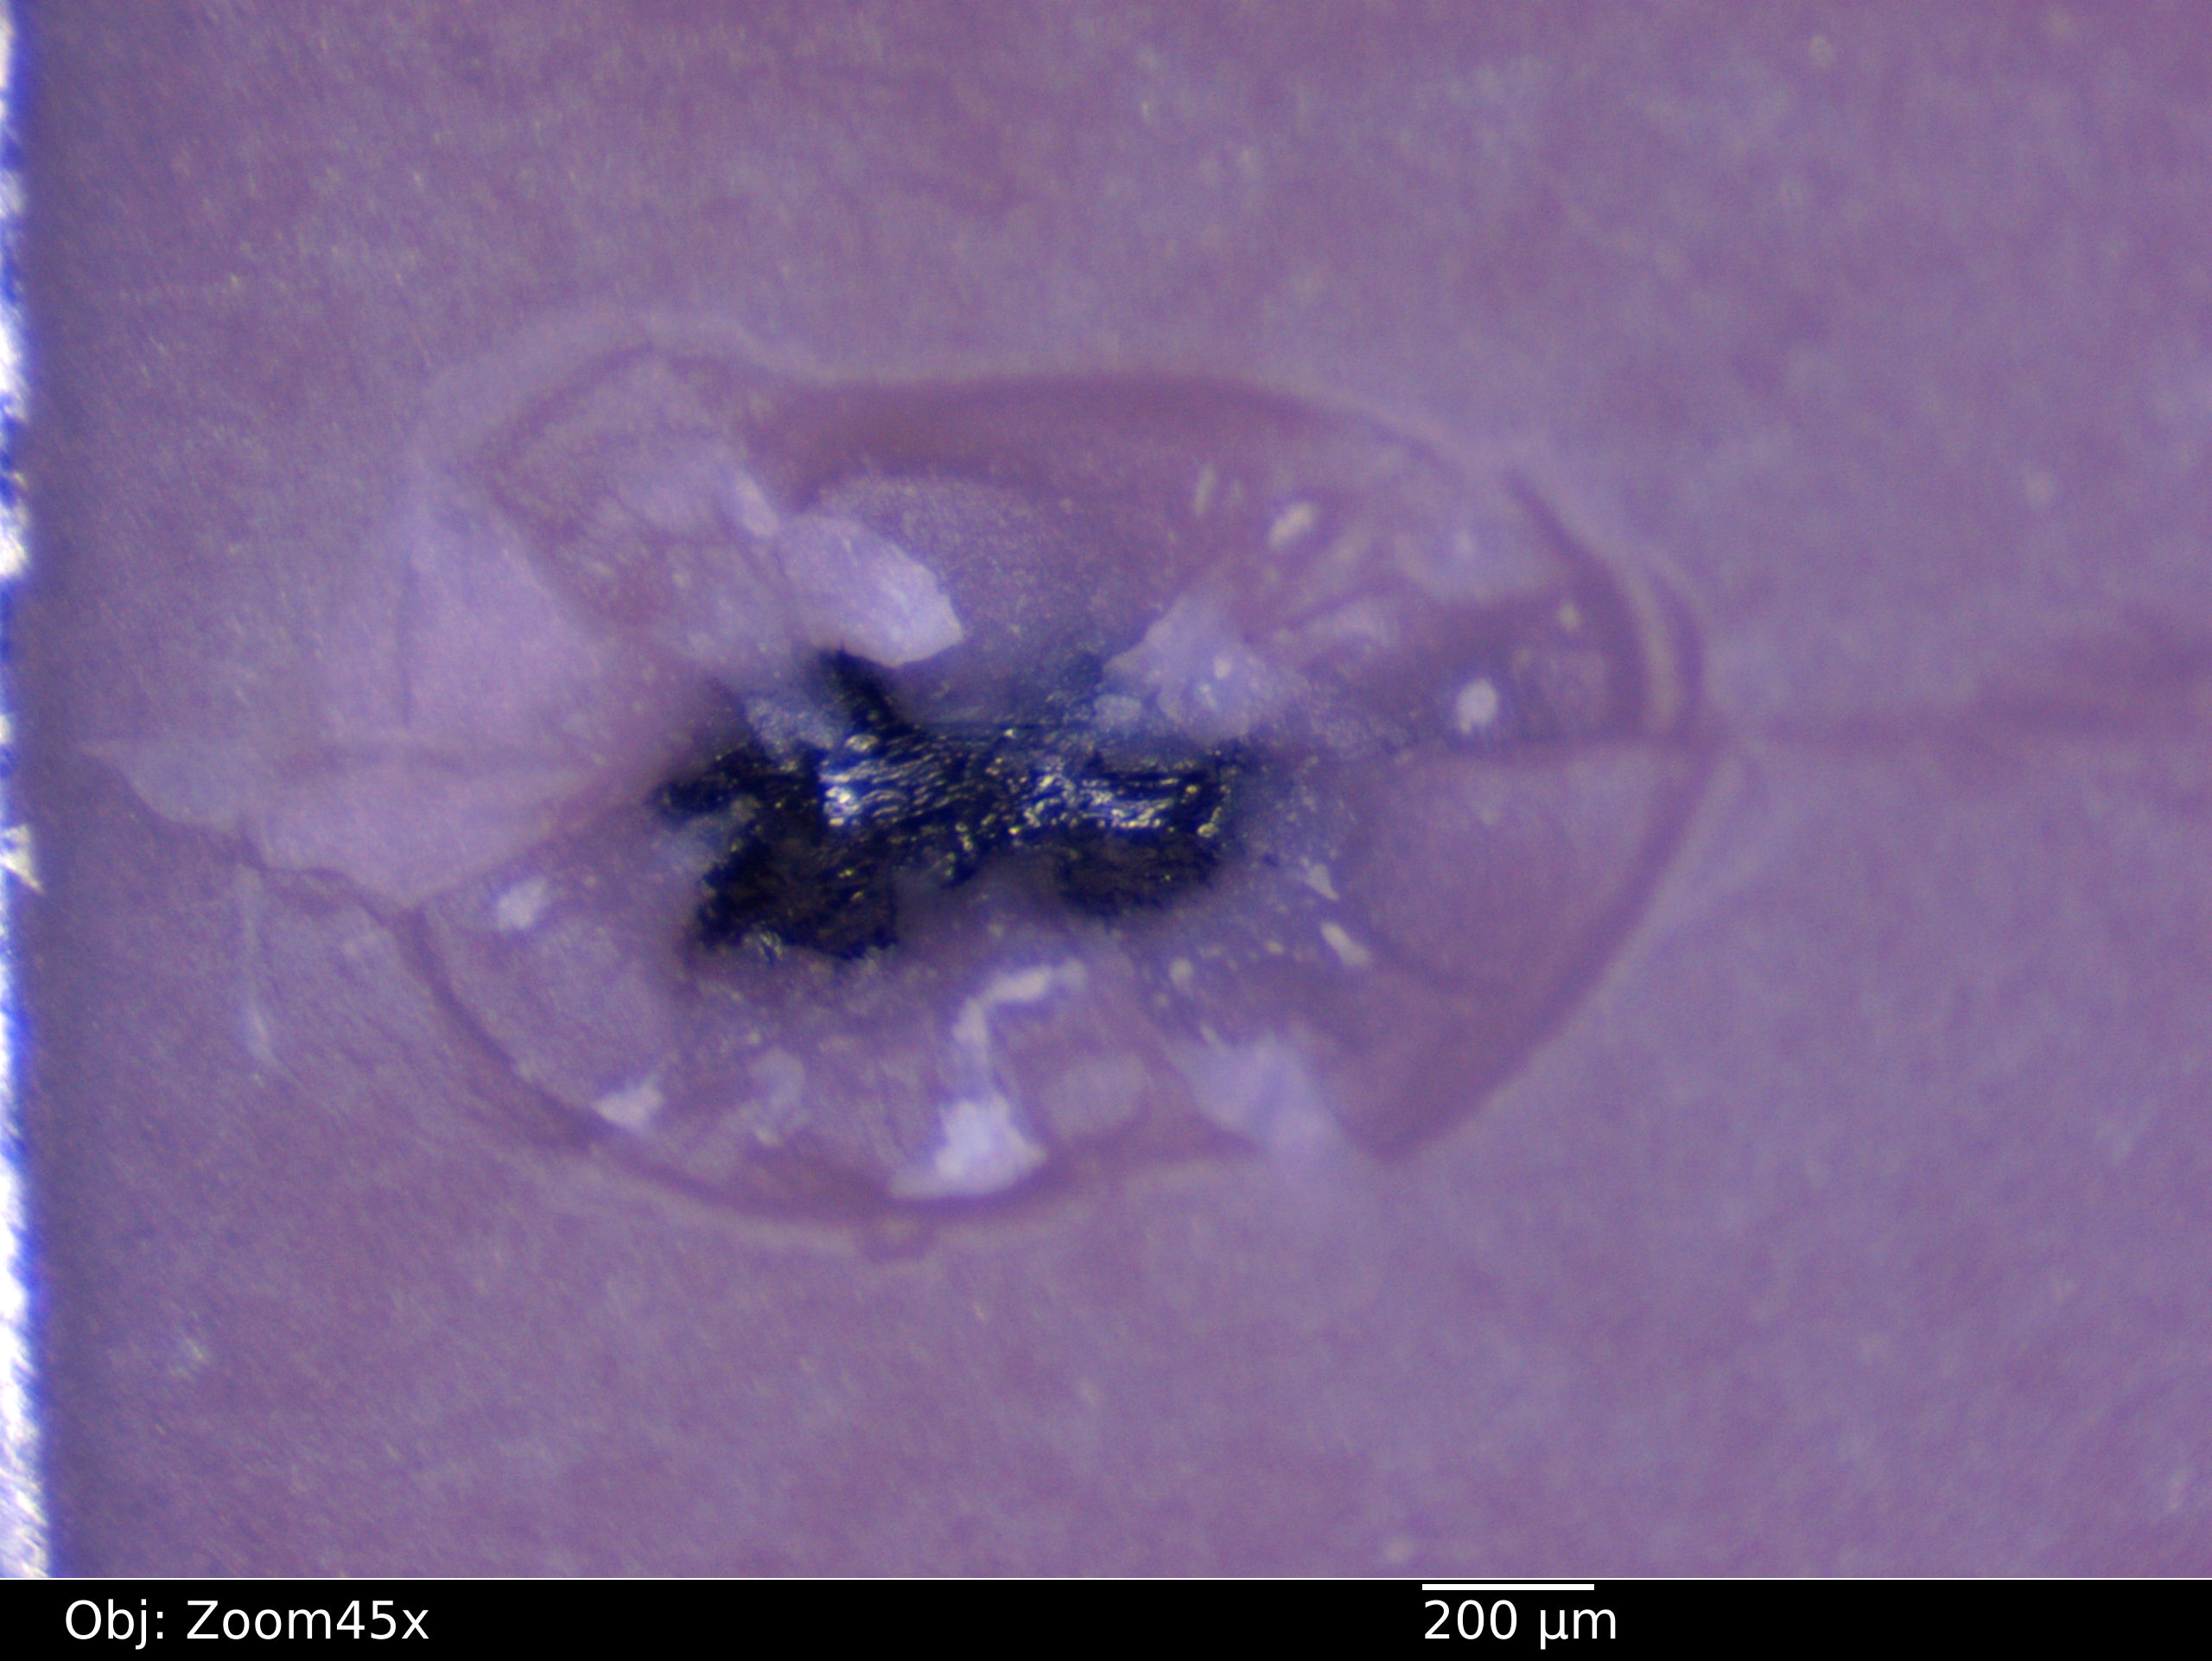
\includegraphics[scale=0.25]{03-badcap-side_annotated.jpg}
\caption{Closeup of failure site}
\label{fail-closeup}
\end{figure}

The large size of the capacitor presented some unique challenges for analysis, since it was too large to fit edgewise
into most standard embedding molds.

Experimentation with using power tools to cut down the test capacitor led to excessive cracking, so bulk material
removal on the actual specimen was performed by hand sanding using 150 and 220 grit aluminum oxide sandpaper.

\end{document}
